\chapter{Casimir effect}\label{cha:casimir-effect}

General introduction and comparison with retarded van der Waals forces

\begin{equation}\label{eq:casimir-pp-force}
  F_\mathrm{Casimir} = - \frac{\hbar c \pi^2}{240 L^4} A
\end{equation}

\begin{equation}\label{eq:casimir-pp-potential}
  V_\mathrm{Casimir} = \frac{\hbar c \pi^2}{720 L^3} A
\end{equation}


Lifshitz:
\begin{equation}
  F_\mathrm{DD} = \frac{\hbar c \pi^2}{240 L^4} \left( \frac{\varepsilon_r - 1}{\varepsilon_r + 1} \right)^2 \varphi(\varepsilon_r)
\end{equation}
\begin{equation}
  F_\mathrm{DM} = \frac{\hbar c \pi^2}{240 L^4} \frac{\varepsilon_r - 1}{\varepsilon_r + 1} \varphi(\varepsilon_r)
\end{equation}

The numeric function $\varphi$ is shown in \cref{fig:casimir-numeric}.


\begin{figure}[!htbp]
  \centering
  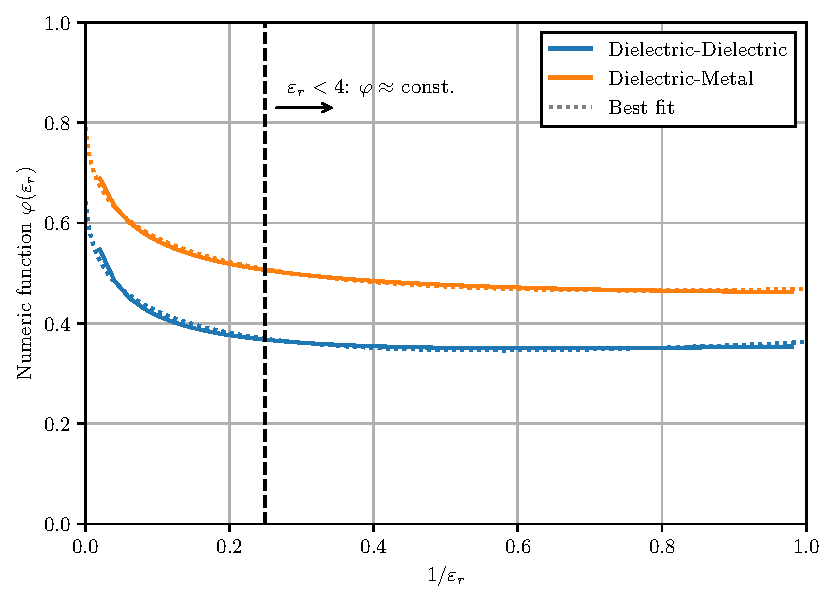
\includegraphics[width=\textwidth]{./../figures/casimir-numeric.pdf}
  \caption{Numeric casimir interaction $\varphi(\epsilon_r)$ between \textbf{(blue)} two dielectric plates and \textbf{(orange)} a dielectric and a conductor.}
  \label{fig:casimir-numeric}
\end{figure}


\section{Proximity force approximation}

\begin{figure}[!htbp]
  \centering
  \def\svgwidth{0.55\textwidth}
  \input{./../figures/proximity-force-approximation.pdf_tex}
  \caption{In the proximity force approximation the sphere is divided into infinitesimal plane areas $\dd A$ which all exert a force $\dd F$ according to eq. \eqref{eq:casimir-pp-force}. All the contributions are added up together.}
\end{figure}





\section{Imperfect plate and spheres}

Python numerical approach, gaussian modes (vibration modes of a spherical plane), perlin noise



\section{Casimir forces between a conducting plate and a dielectric sphere}
\subsection{Polarizability of a dielectric sphere}
The polarizability $\alpha$ is defined via
\begin{equation}
  \vec{E_\infty} \alpha = \vec{p},
\end{equation}
where $\vec{p}$ is the induced dipole moment and $\vec{E_\infty}$ is the external electric field that induces the dipole moment. For a linear and uniform dielectric, it is given as $\vec{p} = \mathcal{V} \varepsilon_0 (\varepsilon_r - 1) \vec{E_\mathrm{in}}$ \cite[p. 220-226]{Griffiths_2018}. Here, $\mathcal{V}$ is the volume of the object and $\vec{E_\mathrm{in}}$ is the electric field inside the dielectric.
The electrostatic boundary conditions for the problem are given by
\begin{equation}
  V_\mathrm{in} \big|_{r=R} = V_\mathrm{out} \big|_{r=R} 
  \quad \text{and} \quad 
  \varepsilon_r\varepsilon_0\pdv{V_\mathrm{in}}{r}\bigg|_{r=R} = \varepsilon_0\pdv{V_\mathrm{out}}{r} \bigg|_{r=R}
\end{equation}
and the electric potential outside of the sphere at $r\rightarrow\infty$ should be equal to the external dipole-inducing field $V_\mathrm{out} |_{r\rightarrow\infty} = -\vec{E_\infty} \cdot \vec{r} = -E_\infty r\cos\theta$.
The electric potential inside and outside the sphere can be calculated using the spherical decomposition of the general electric potential $V \propto 1/\abs{\vec{r} - \vec{r'}}$ into Legendre Polynomials $P_l$ \cite[p. 188-190]{Griffiths_2018}:
\begin{align}
  V_\mathrm{in}(r, \theta) &= -E_\infty r\cos\theta + \sum_{l=0}^{\infty} A_l r^l P_l(\cos\theta), \\
  V_\mathrm{out}(r, \theta) &= -E_\infty r \cos\theta + \sum_{l=0}^{\infty} \frac{B_l}{r^{l+1}} P_l(\cos\theta).
\end{align}
Applying both boundary conditions, it follows that \cite[p. 249-251]{Griffiths_2018}
\begin{equation}
  \begin{cases}
    A_l = B_l = 0 & \text{for } l \neq 1, \\
  A_1 = -\frac{3}{\varepsilon_r + 2}E_\infty, \quad B_1 = \frac{\varepsilon_r-1}{\varepsilon_r + 2}R^3E_\infty
  \end{cases}
\end{equation}
and the resulting  homogenous electric field $\vec{E_\mathrm{in}} = -\vec{\nabla} V_\mathrm{in}$ inside the sphere is given as
\begin{equation}
  \vec{E_\mathrm{in}} = \frac{3}{\varepsilon_r + 2} \vec{E_\infty} .
\end{equation}
The field is shown on the right in \cref{fig:dielectric-sphere-field}.The polarizability $\alpha$ of the sphere can be now be determined to
\begin{equation}
  \alpha_\mathrm{sphere} = 4\pi \varepsilon_0 R^3 \left(\frac{\varepsilon_r - 1}{\varepsilon_r + 2}\right).
\end{equation}

% \begin{figure}[!htbp]
%   \centering
%   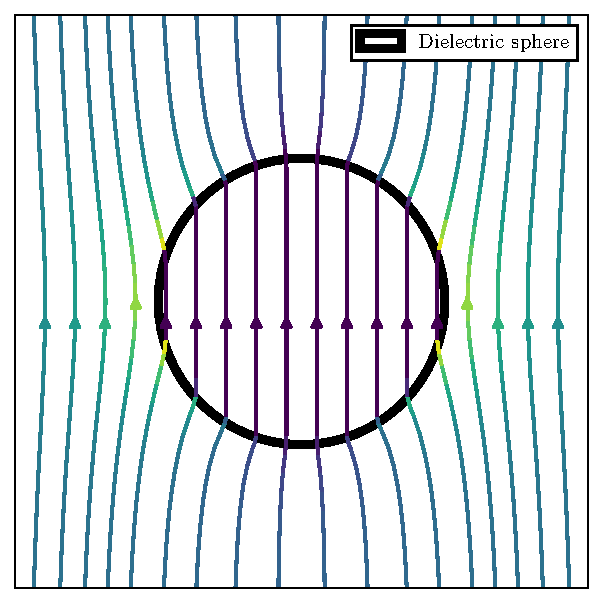
\includegraphics[width=0.8\textwidth]{./../figures/field-dielectric-sphere.pdf}
%   \label{fig:field-dielectric-sphere}
%   \caption{Electric field lines through an dielectric sphere}
% \end{figure}

\begin{figure}[!htbp]
  \centering
  \begin{subfigure}[b]{0.48\textwidth}
      \centering
      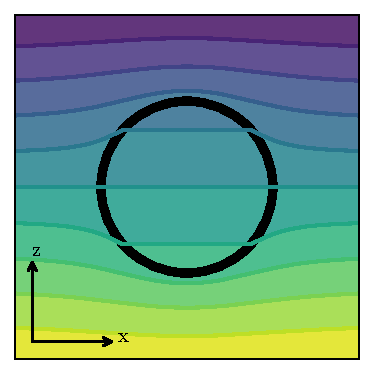
\includegraphics[width=\textwidth]{./../figures/potential-dielectric-sphere-small.pdf}
  \end{subfigure}
  \hfill
  \begin{subfigure}[b]{0.48\textwidth}
      \centering
      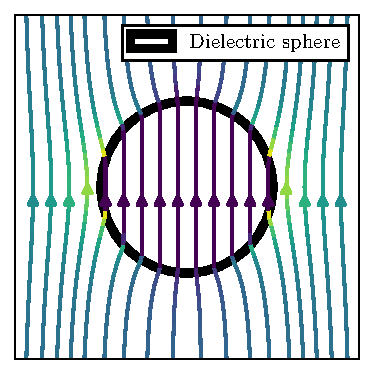
\includegraphics[width=\textwidth]{./../figures/field-dielectric-sphere-small.pdf}
  \end{subfigure}
  \caption{\textbf{left:} Electric potential $V$ of a dielectric sphere in a external electric field $\vec{E_\infty} \parallel \vec{e_z}$. \textbf{right:} The corresponding electric field lines inside and outside the dielectric sphere.}
  \label{fig:dielectric-sphere-field}
\end{figure}